\chapter{Processing the Captured Data}
This chapter is dedicated to the process of extracting critical data from the video files and the smartphone csv file. This process will take the raw captured data and transform it to values that we can feed into the Extended Kalman Filter. It is referred to in this work as preprocessing since the data is being processed before the filter.

\section{Processing the IMU Data}
The following flowcharts depicts the procedural processing of smartphone sensor and GPS data gathered from the chest mounted smartphone running the AndroSensor application. The following flow diagram shows the different steps in preprocessing.

\begin{figure}[!ht]
\captionsetup{width=0.8\linewidth, font=small}  
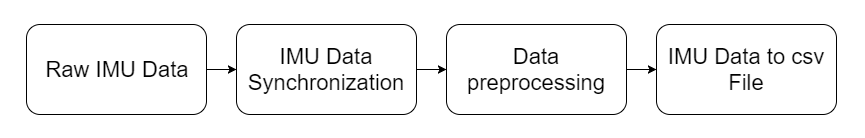
\includegraphics[width=\linewidth]{figures/imuflow.png}
\caption{Diagram showing the progression and dependence of the major stages of sensor data processing in this project}
\label{fig:imuflow}
\end{figure}

From the diagram our raw input log file is a large unprocessed dataset captured by the smartphone with a logging rate of 100Hz. From this the critical data must be extracted and synchronized with the rest of the system. The data must also be manipulated to keep units constant and unify various frames of reference. By correctly preprocessing the data, the implementation of the EKF is simplified.

\subsection{Obtaining IMU Data}
Obtaining the raw sensor data was discussed in the previous chapter. The AndroSensor application was configured by specifying the units that all sensors must be logged in. The units of each sensor was selected as per the table below.

\begin{table}[!ht]
\centering
\captionsetup{width=0.8\linewidth, font=small}  
\caption{Table showing the different units of the output AndroSensor file}
\label{Smartphone Data Units}
\begin{tabular}{ll}
Heading               & Units  \\
ACCELEROMETER       & $ m/s^2 $  \\
GRAVITY              & $ m/s^2 $ \\
LINEAR ACCELERATION  & $ m/s^2 $\\
GYROSCOPE            & $ rad/s $ \\
MAGNETIC FIELD       &  $  microTesla$\\
ATMOSPHERIC PRESSURE  &     $ Pascal$ \\
LOCATION Latitude     &    $ degrees $   \\
LOCATION Longitude    &    $ degrees $   \\
LOCATION Speed        &     $ m/s $  \\
LOCATION ORIENTATION  &     $ degrees $  \\
VOLUME				&		$ dB $
\end{tabular}
\end{table}

The importance of having uniform units is discussed later in this chapter. The above units have been chosen since they are SI units or the most relevant next possibility.

\subsection{Synchronizing IMU Data}
Previously the application used by \cite{bradstocks} created a beep tone when the logging process was started. This beep tone was recorded by the cameras and was used as a common point of synchronization. Some drawbacks were identified by using this method. The smartphone would start logging only after the beep had completed. this meant that the smartphone data had to be resynchronized to the camera data by further testing. Another shortcoming was that the beep tone was not loud enough to comfortably be detected by the rear cameras, causing difficulty in noisy environments.

The AndroSensor application can record the the magnitude of sound that the microphone is experiencing at a given time. Using this magnitude we can see at what time instance a spike in volume (caused by a simple clap of the hands) was logged. This sample can be a common point between the IMU and the cameras and can thus be used to synchronize the different hardware elements.

Upon further consideration a point of synchronization should be created before and after the testing period to ensure that the different data streams stay in sync. This meant that volume spike had to be made before and after each run. 

\subsection{Preprocessing IMU Data}
All these variables have been recorded with respect the smartphone frame of reference. Since the smartphone was rigidly mounted to the body, a simple axis transformation could be completed to move the data onto the body frame of reference. This is further discussed in a following section.

Before we can input the sensor data directly to the EKF, we need to make some minor modifications to the data. This includes zeroing the positional data given by the GPS, since we assume our subject to start at position $ (0,0) $ in the inertial frame. To zero the the following formulae was applied.

$$  gps lat = ( gps lat -  gps lat_i)\times 110922 $$
$$  gps long = ( gps long -  gps long_i)\times 92423 $$

These algorithms subtracts the initial value of the GPS latitude and longitude from every value in the data vector and multiplies the difference by scalars to move the points to a NED frame of reference. These scalar values where obtained from \cite{gps}.
  
$$  gps vel x =  gps speed \times \cos( gps head) $$
$$  gps vel y =  gps speed \times \sin( gps head) $$

The above algorithms compute the x and y components from the GPS velocity vector by using the magnitude and heading logged from the sensor.

The accelerometer and gyroscope also contained some bias. This can be quantified by logging a large dataset while the smartphone is absolutely stationary and finding the average non-zero value of the individual sensors. Calculating the bias vectors we find them to be. For the accelerometer these values have been calculated as:

$$accelerometer X = -2.74252 \times 10^-5	m/s^2 $$
$$accelerometer Y = -2.61902 \times 10^-5	m/s^2 $$
$$accelerometer Z = 2.04709  \times 10^-5	m/s^2 $$

The values for the gyroscope has been calculated as:

$$gyroscope X = 5.46604 \times 10^-5	r/s $$	
$$gyroscope Y = 1.29292 \times 10^-5	r/s $$		
$$gyroscope Z = 2.87219 \times 10^-5	r/s $$ 

The logged data was modified to subtract these bias values.
 
\subsection{Exporting IMU Data}
The IMU data was finally exported as a final csv file and imported into MATLAB as a set of vectors. Each vector containing the samples of a specific data field. This allows for faster processing and access to the data.

The final step was to compute availability vectors for all the different data fields. This was done by creating a vector that contains a 1 if the sensor value has changed and a 0 if the value has not updated. Since many of the sensors on the smartphone do not update at 100Hz this was necessary to only input the values to the EKF if there was an update. When analysing these availability vectors we can see that the barometer only updates at a rate of 5Hz and the GPS at a rate of 1Hz.

\newpage
\section{Processing the Video Data}
To further simplify the design and implementation of the EKF it is important to pre-process the video data to a less data heavy format than MP4. The following digram shows the process of converting a large video file to a more lightweight csv file without losing any critical information.

\begin{figure}[!ht]
\captionsetup{width=0.8\linewidth, font=small}  
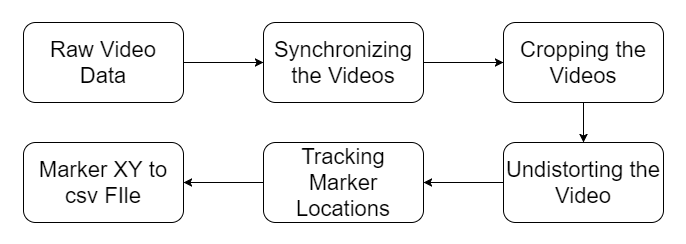
\includegraphics[width=\linewidth]{figures/videoProcess.png}
\caption{Diagram showing the progression and dependence of the major stages of video processing in the project}
\label{fig:videoProcess}
\end{figure}

All raw video data streams must be synchronized and the important sections of the streams extracted. Correcting the various distortions introduced by the lens properties of the GoPro and decompressing the video files are necessary before image processing is attempted. Finally each marker position in every frame of all the individual cameras must be quantified. These pixel coordinates will serve as inputs to the EKF. 

\subsection{Obtaining Video Data}
The cameras were housed in the custom designed dual camera housing shown in the previous chapter. Two cameras at the front capturing the motion of the lower limbs when they have a positive hip angle and two cameras mounted to the back to capture negative hip angles.

The GoPro cameras were all connected to a single GoPro remote and configured to record video when the remote was activated. After the harness had been properly secured the cameras were started. The remote starts the cameras at similar times, but not accurately enough to use as a method of synchronization. Below is a picture of the GoPro remote used.

\begin{figure}[!ht]
\captionsetup{width=0.8\linewidth, font=small} 
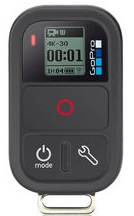
\includegraphics[width=0.1\linewidth]{figures/remote.jpg}
\caption{GoPro camera remote control}
\label{fig:remote}
\end{figure}

\subsection{Synchronizing Video Sources}
I typical problem faced when working with different sources of data is that of synchronization. Since this project ases 4 different cameras, synchronizing the video sources are critical to generate accurate stereo vision and lower limb data.

The problem of synchronization was overcome by using a audio cue to align the video data post capturing. With all systems recording, a simple hand clap can serve as a spiking audio input easily identified in the audio track of the video streams. The frame associated with this audio spike can be identified using SVP (Sony Vegas Pro) video editing software as shown in the figure below. 

\begin{figure}[!ht]
\captionsetup{width=0.8\linewidth, font=small} 
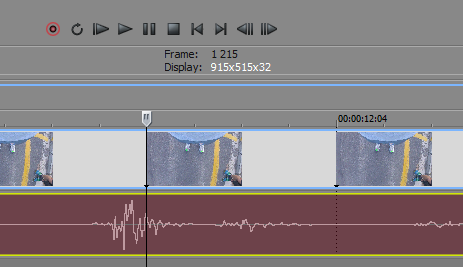
\includegraphics[width=0.5\linewidth]{figures/svpframe.png}
\caption{Figure showing the user interface of SVP video editing software}
\label{fig:svpframe}
\end{figure}

The red track in the above figure shows the recorded audio stream while the corresponding frames are displayed in the blue track above that. The cursor is aligned with the audio spike caused by the clap with the corresponding frame number displayed below the playback controls. This method was repeated for every video stream such that a common starting point was generated. 

\subsection{Cutting Critical Video Data}
With the video data synchronized the next step was to generate a subset of video demonstrating a transient period and steady state period of running. By inspecting the videos we can identify the different phases of the run and we can extract their frame numbers by once again using SVP.

A single video was used to determine the different points of the run. From synchronization to the end of the run was 18 seconds. This quantifies as 1800 frames as the cameras are recording at 100 frames per second.

A MATLAB script was created to cut the 1800 critical frames from the raw video file. This script also uncompressed the video files to a more data intensive .AVI file that contains a RGB vector for each individual pixel. The decompression of the video files makes them easier to manipulate as objects in MATLAB, but does however not restore any of the data lost in the process of compression. This MATLAB script can be found on the accompanying CD.

\subsection{Undistorting the Video Data}
Due to the intrinsic lens properties of the GoPro cameras the edges of each frame had been severely distorted. To gain further understanding of undistorting video files \cite{Hartley2004} served as a reference. By using The built in camera calibration toolbox in MATLAB we can generate the various camera matrices needed to undistorted the video files.

A custom MATLAB script was created to undistort the critical video segments. This script used the camera matrix in conjunction with build in functions to correct the lens distortion frame by frame of each video stream. The script can be found on the accompanying CD. The following image shows the difference before and after the frames were corrected.

\begin{figure}[!ht]
\captionsetup{width=0.8\linewidth, font=small} 
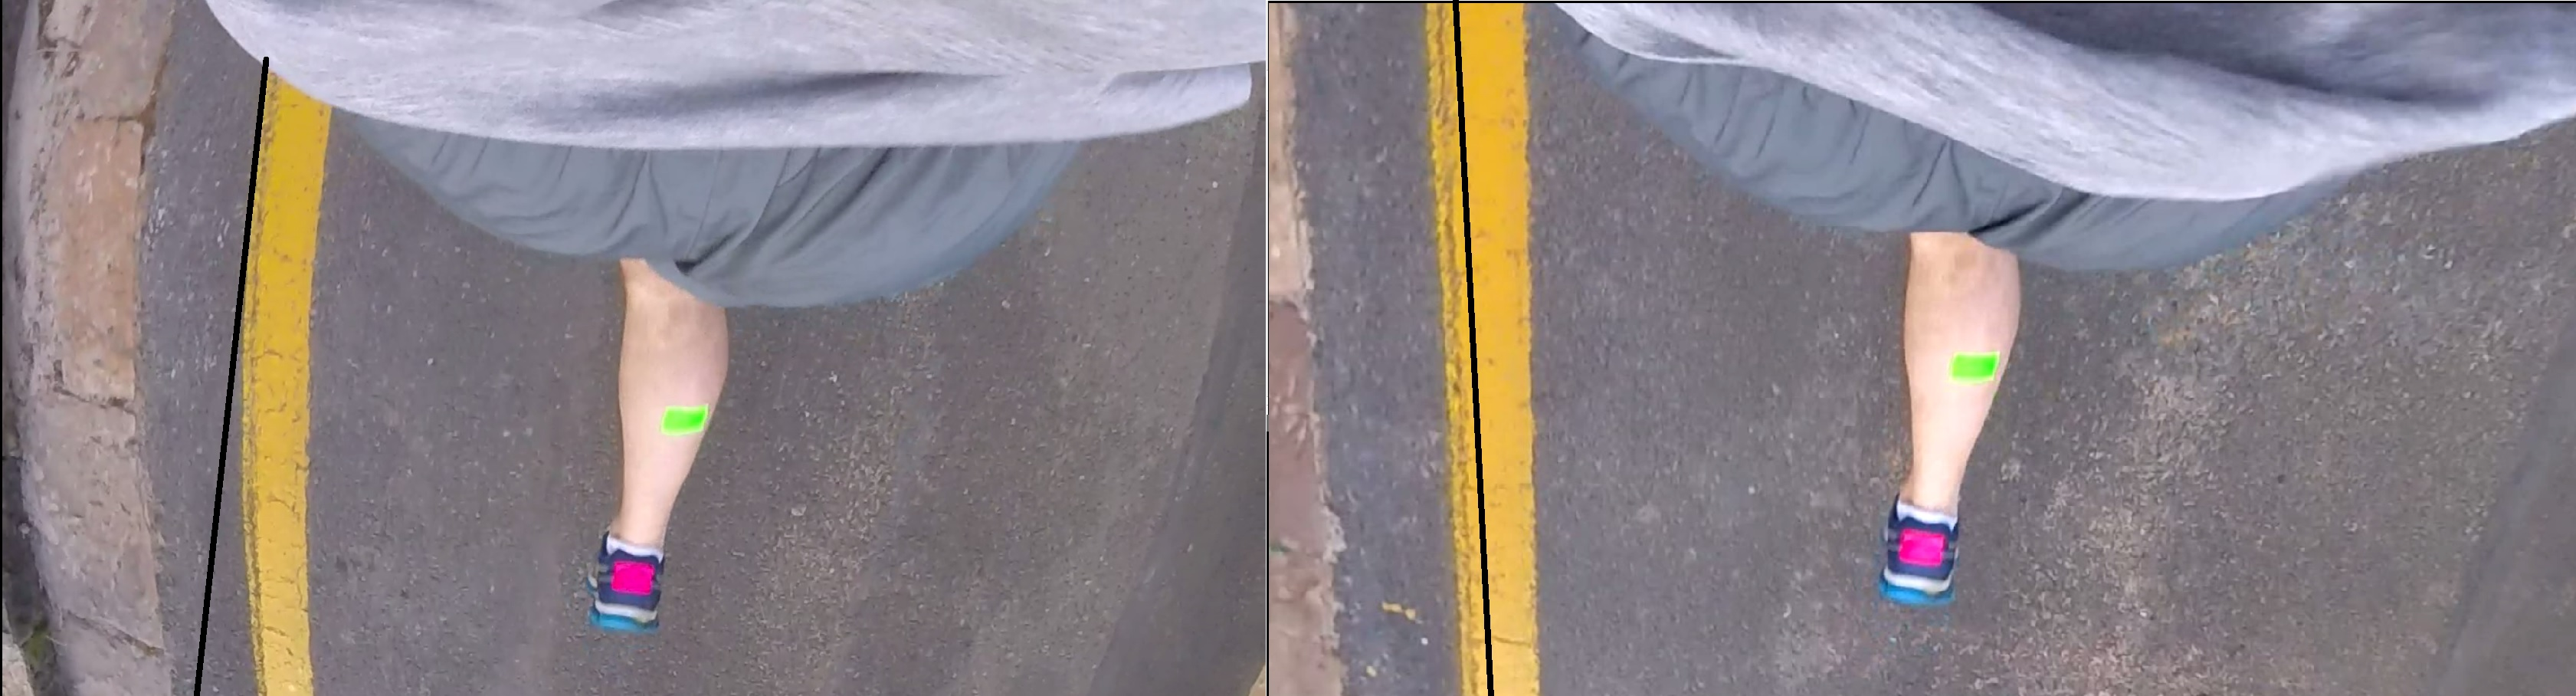
\includegraphics[width=\linewidth]{figures/fixed.jpg}
\caption{Images demonstrating the effects of lens distortion.}
\label{fig:fixed}
\end{figure}


\subsection{Tracking and Exporting Marker Positions}
This section discusses the different methods of image processing subdividing them into two main methodologies: automated and semi-automated. Each of these approaches offer advantages and disadvantages. To understand the approaches considered for this work it is important to visualize the input image data to the system. The following picture shows the various frames from all the cameras.

\begin{figure}[!ht]
\captionsetup{width=0.8\linewidth, font=small} 
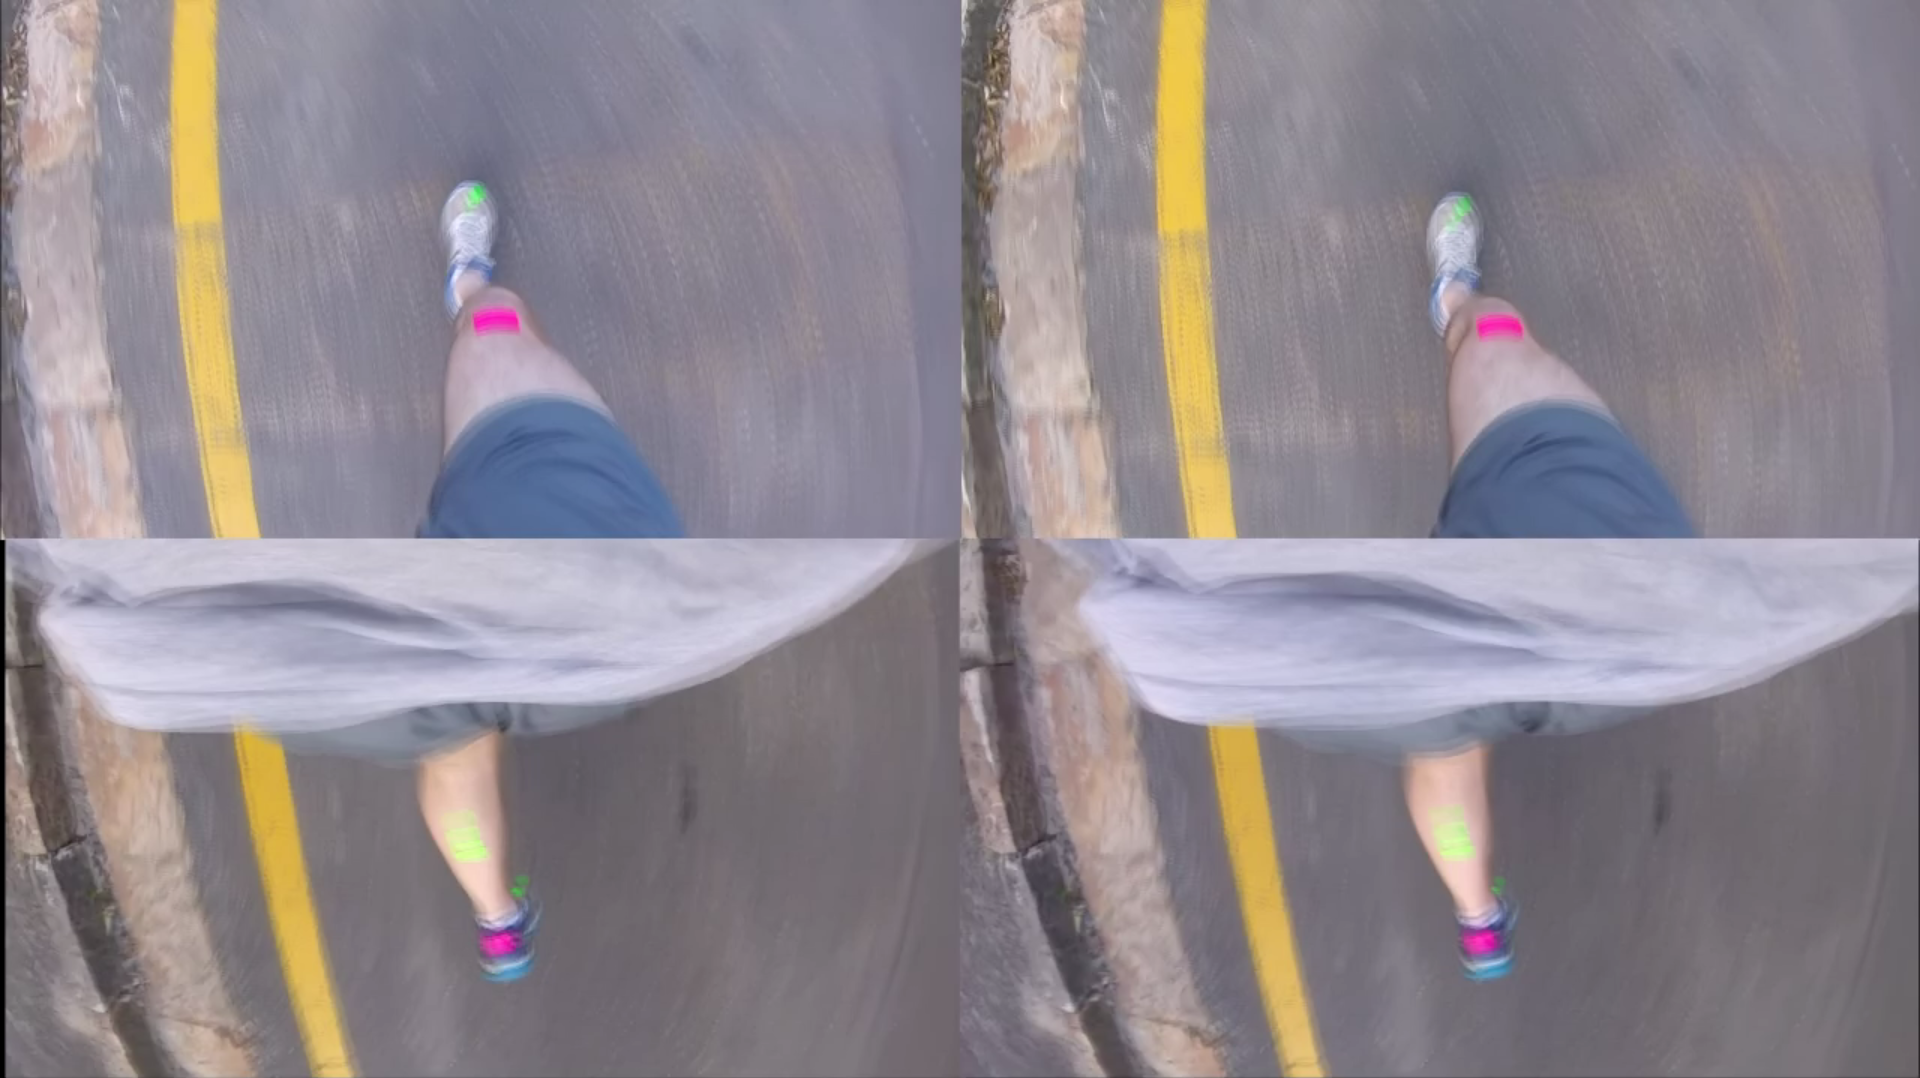
\includegraphics[width=\linewidth]{figures/pat_run_quad.png}
\caption{4 Frames from the different cameras combined}
\label{fig:pat_run_quad}
\end{figure}

The top row of images have been generated by the front mounted cameras and the bottom row by the rear mounted cameras. The left images were produced by the left cameras and the right images by the right cameras. From this image we can get a visual idea of the data our image processing system needs to manipulate.

Feature detection is a methodology in image processing that allows critical points of an image to be detected. This extracts an XY coordinate of the point of interest that can then be used to track the movement and position of an object in the image. This methodology can be applied to frames with more than one point of interest as shown in this work. Multiple points of interest in multiple video sources does however increase the complexity of feature detection.

An initial approach of using automated detection was chosen and three possible system were considered. Using a trained \textit{neural network}, using an \textit{edge detection} algorithm with a panning search algorithm and finally using a \textit{colour identifying} algorithm paired with a local search algorithm. These approaches all require a considerable amount of software to implement and therefore the viability of each has to be considered.

In theory a well trained \textit{neural network} will provide the most robust and accurate system to identify features in varying lighting condition. It would also be the most accurate methodology for a system without the markers. This is due to the "understanding" developed by the neural network after sufficient training data is processed. Strong choices for neural network types would be a Hopfield network or a feed-forward network.

Training a network presents a key difficulty in setting up a neural network. The most important element of a neural network is the training data used to teach the network the correct node weightings. Training data consist of annotated images with descriptive metadata. Such a dataset needs to be created either automatically using image processing algorithm or can be created by computer assisted image processing. A neural network therefore cannot generate its own training data and can therefore only be used as a semi automated identification system.

The second approach considered was that of \textit{edge detection}. This method identifies various edges in the image using discontinuities in brightness. Such a system can easily detect the edges of a marker, but cannon differentiate or classify edges. Pairing edge detection with a panning search algorithm allows us to search for marker shaped objects post edge detection. This algorithm needs to correctly identify the marker shapes and correctly differentiate and uniquely annotate the different markers as their respective points.

Although the implementation of edge detection is rather trivial, creating a search algorithm that can correctly identify changing marker shapes and assign them their correct point classification seems beyond the scope of this project. The following image shows edge detection as applied to a camera frame.

\begin{figure}[!ht]
\captionsetup{width=0.8\linewidth, font=small} 
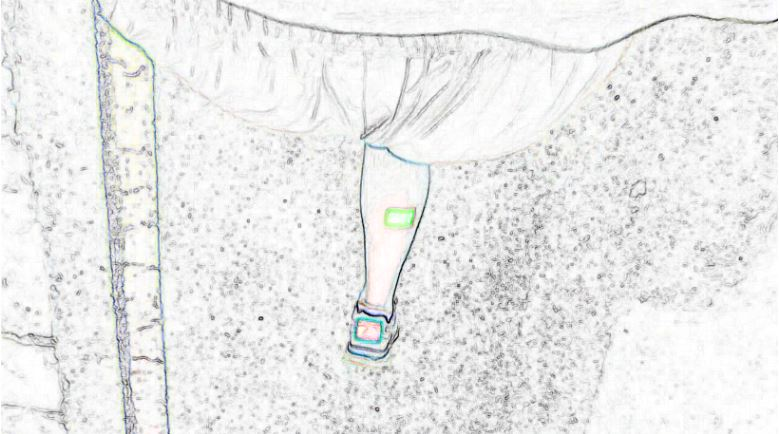
\includegraphics[width=0.6\linewidth]{figures/ed.jpg}
\caption{4 Frames from the different cameras combined}
\label{fig:ed}
\end{figure}

From this example we can see that the marker edges are correctly identified, but the colours do not correlate. As assumed the difficulty in this approach is not creating the image processing algorithm but rather in creating a panning search algorithm to extract marker information.

Another approach considered was that of a \textit{colour identifying} algorithm. By using such methods the markers with their bright colours are easy to identify and differentiating between pink and green markers also seem trivial. The local search algorithm is also easy to implement and will start searching for marker in the next frame at the coordinates of the same marker identified in the previous frame. 

Such an approach was partially implemented, but did not provide consistent enough results to use. These inconsistencies arise from the GoPro camera automatically adjusting its light level to best suit the environment. Changing the recorded light levels changes the perceived RGB values of the markers. This forces us to increase the colour rage of our markers, introducing more uncertainty and increasing the possibility false positives.

Another major drawback to using such a system is that it is not a generalized solution. This implies that the same markers must be used at the same positions every time the experiment is run. It also depends heavily on the markers, stunting the idea of transitioning to a markerless system.

By comparing the proposed automatic methods above and considering ease of implementation and accuracy no single method seems viable. This is either due to the lack of example data (in the case of the neural network), or the limitations of computer algorithms (too complex in the case of edge detection and not general purpose or accurate enough in the case of the colour identifier).

\newpage
The final approach considered and used was to \textit{semi automatically} label critical point in the image using a toolbox created by Hedrick et al. \cite{hedrick2008software}. This software allows for a semi automatic tracking of points of interest in the video frames by using user input in conjunction with computer algorithms. While this method is labour intensive it is arguably more accurate than the previously investigated methodologies and more generalized. The following figure shows the functionality of the toolbox within MATLAB.

\begin{figure}[!ht] 
\captionsetup{width=0.8\linewidth, font=small}  
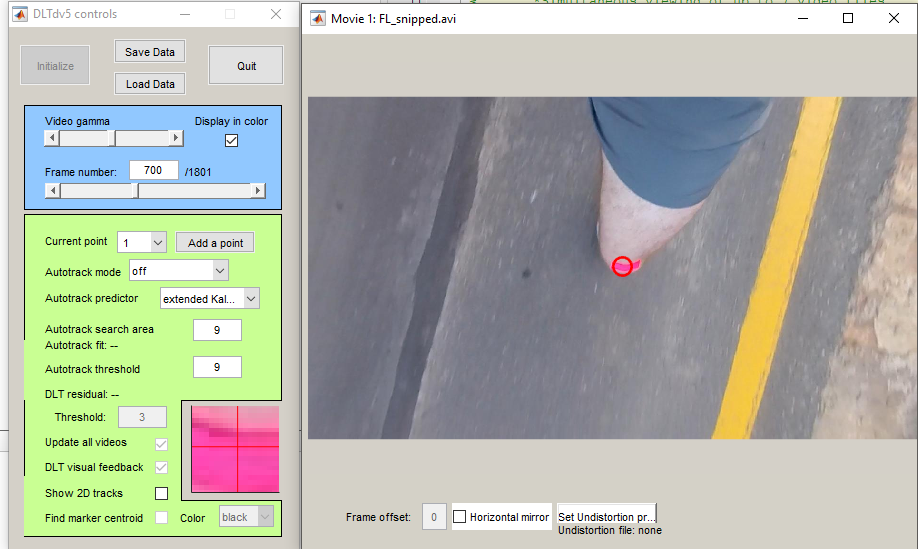
\includegraphics[width=0.5\linewidth]{figures/toolbox.png}
\caption{Using the dltdv toolbox in MATLAB to export marker coordinates}
\label{fig:toolbox}
\end{figure}

By using this toolbox we can generate a dataset of $ (x,y) $ pixel coordinates by identifying the different markers on each frame and assigning their corresponding points to them. The following tables shows the markers and their corresponding point.

\begin{table}[!ht]
\centering
\caption{Table showing the relation between points and markers}
\label{my-label}
\begin{tabular}{lll}
Point & Identifier           & Marker Colour\\
Front Cameras &            &\\
Point 1       & Right Knee &PINK \\
Point 2       & Left Knee  &PINK\\
Point 3       & Right Foot &GREEN\\
Point 4       & Left Foot  &GREEN\\
Rear Cameras  &            &\\
Point 1       & Right Calf&GREEN \\
Point 2       & Left Calf &GREEN \\
Point 3       & Right Heel&PINK \\
Point 4       & Left Heel &PINK \\
\end{tabular}
\end{table} 

Each video stream was processed and a total of 16 different coordinate sets was generated, 8 from the front cameras and 8 from the rear cameras. These coordinates were output as csv files that could easily be imported into MATLAB.


Finally availability vectors were created for each of the 16 points. 
From these vectors we can also calculate the percentages of each camera seeing each marker. This can give us an idea as to how often the cameras are contributing data and how much of the total gait is captured. These percentages are discussed in a following chapter.

\section*{On units}
In order to assure consistency between the different sources of data considering a general set of units is of critical importance. It was decided to implement the system using SI units such that all lengths was given in meters and all angles in radians.

\section*{On Frames of Reference}
we need to developed some commonalities among the various sensors and their individual frames of reference. This thesis considers 4 different frames of reference, namely: the body frame, the smartphone frame, the camera frame and the inertial frame.

The body frame has been defined as shown in the image below.

\begin{figure}[!ht] 
\captionsetup{width=0.8\linewidth, font=small}  
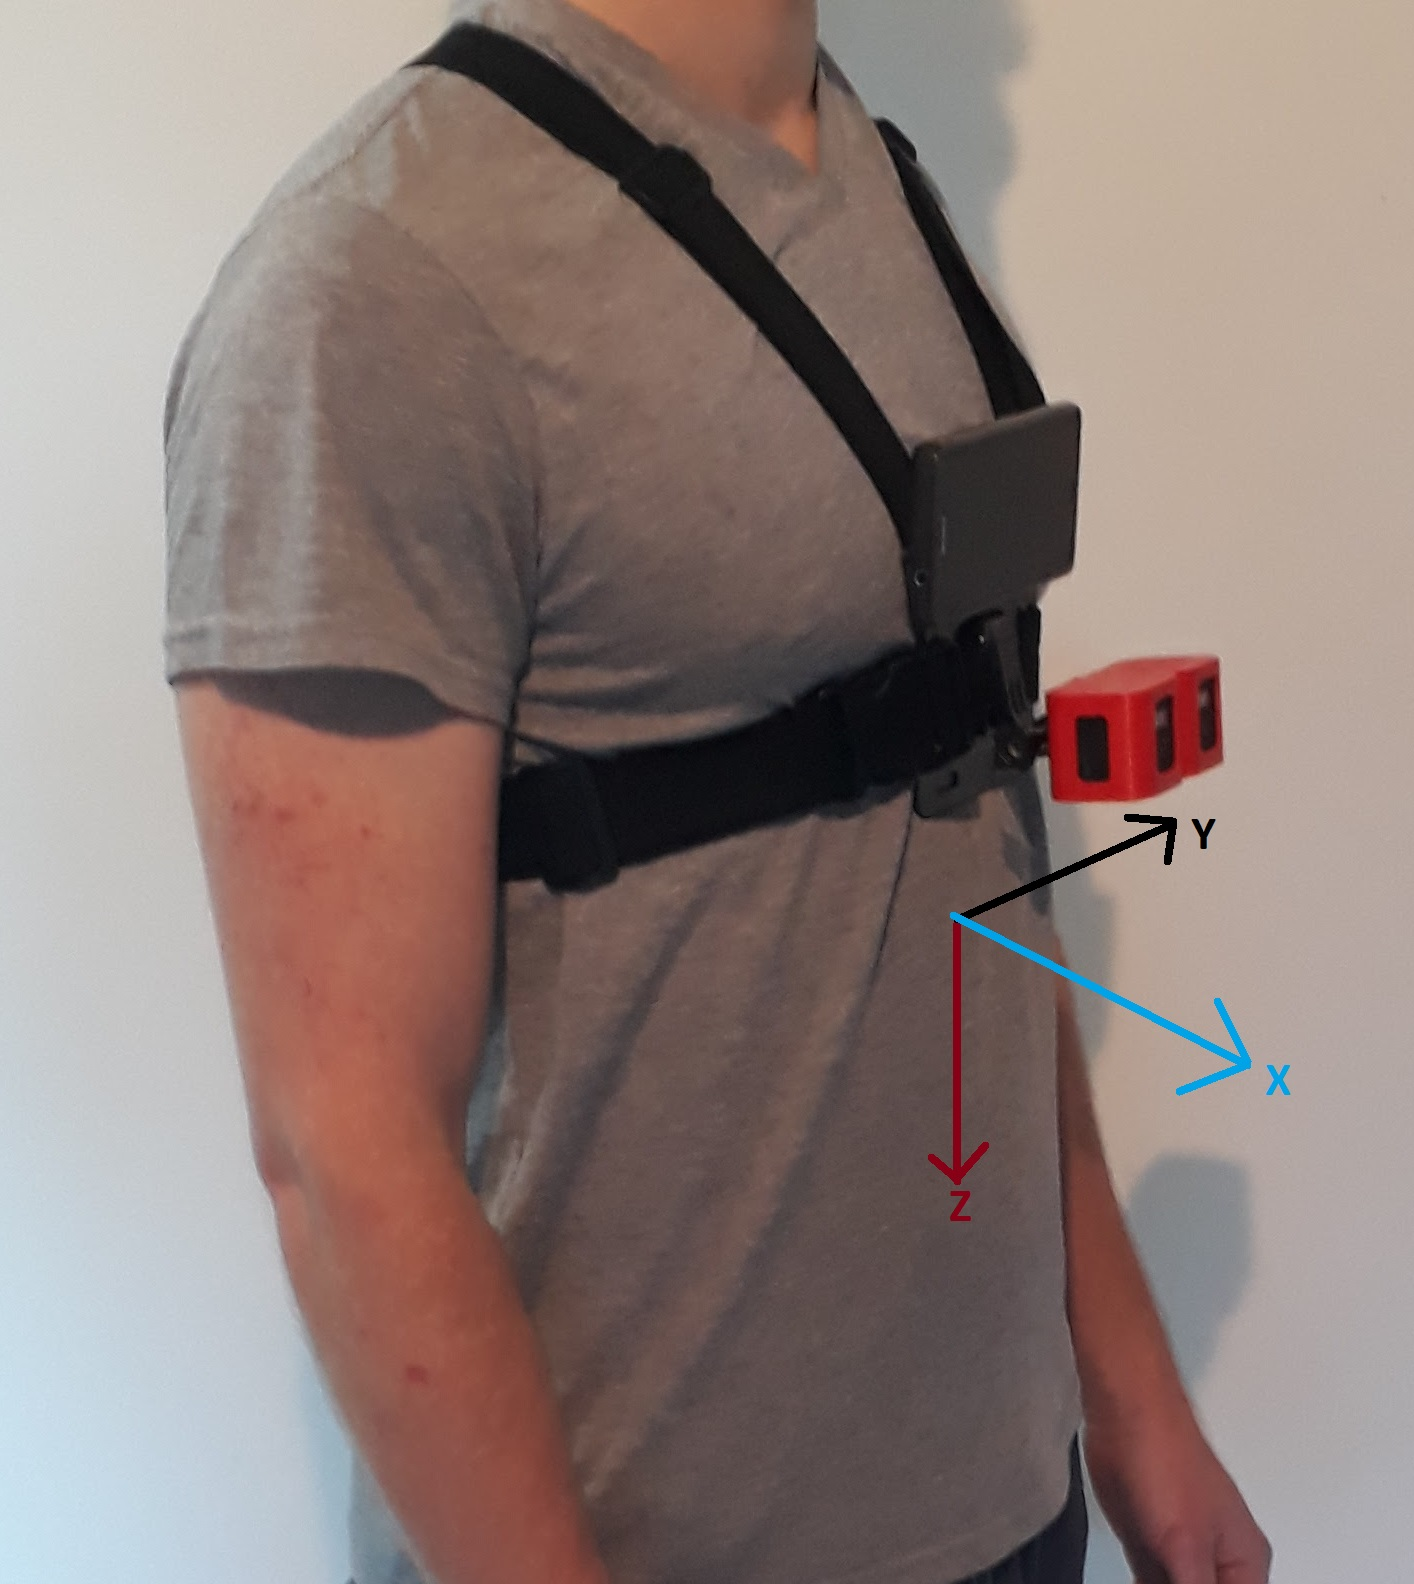
\includegraphics[width=0.5\linewidth]{figures/patbf.jpg}
\caption{Figure demonstrating the body frame of reference}
\label{fig:patbf}
\end{figure}

The smartphone frame is shown in this image below.

\begin{figure}[!ht] 
\captionsetup{width=0.8\linewidth, font=small}  
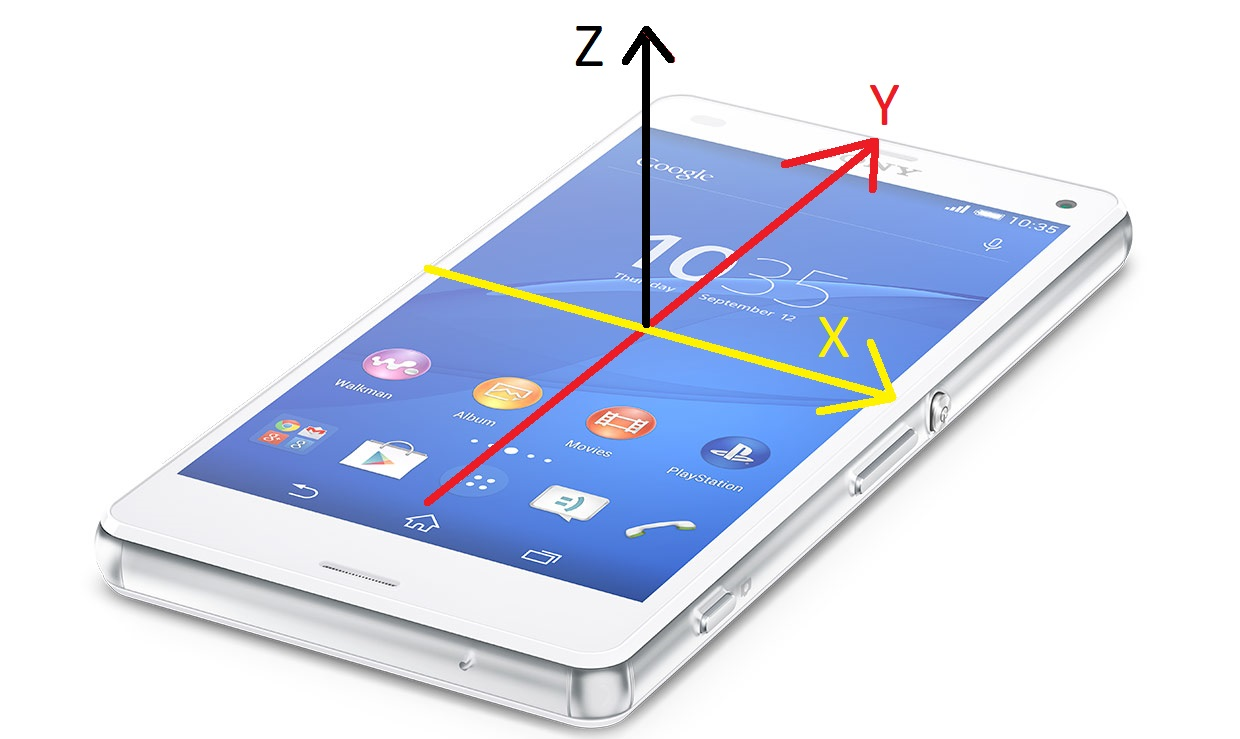
\includegraphics[width=0.5\linewidth]{figures/phone.jpg}
\caption{Figure demonstrating the frame of reference of the smartphone}
\label{fig:phone}
\end{figure}

Since the smartphone is rigidly mounted to the body a simple axis transformation is required to transform the sensor data to the body frame. The following equations shows the transformation.

$$ bodyX = smartphoneZ  $$
$$ bodyY = -smartphoneY  $$
$$ bodyZ = -smartphoneX  $$

There is however another frame of reference that is important to understand, that of the camera frame.

\begin{figure}[!ht] 
\captionsetup{width=0.8\linewidth, font=small}  
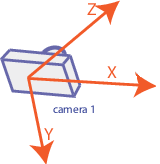
\includegraphics[width=0.5\linewidth]{figures/cf.png}
\caption{Figure demonstrating the camera frame of reference, image adapted from \cite{matlab}}
\label{fig:cf}
\end{figure}

Since the cameras are pointing down when the subject is standing still the Z axis of the camera aligns with the Z axis of the body. The X and Y axis are transformed during fusion.














